\documentclass[aspectratio=169]{beamer}

\usetheme{default}
\setbeamercolor{background canvas}{bg=white}
\setbeamercolor{structure}{fg=black}
\setbeamercolor{normal text}{fg=black}
\setbeamertemplate{navigation symbols}{}
\setbeamertemplate{footline}{}

\usepackage{tikz}
\usepackage{listings}
\usepackage{algorithm2e}

\RestyleAlgo{plain}
\DontPrintSemicolon
\SetKwInOut{Input}{input}
\SetKwInOut{Output}{output}

% vnv.png is reused from the intro lecture rather than copied.
\graphicspath{{.}{../000-intro/}}

\setbeamertemplate{blocks}[rounded][shadow=false]
\setbeamercolor{block title}{bg=blue!65!black,fg=white}
\setbeamercolor{block body}{bg=blue!8,fg=black}

% Small grey image credit, placed directly under a figure.
\newcommand{\credit}[1]{\par\vspace{0.3em}{\tiny\color{gray}#1}}

\lstdefinestyle{matlab}{
  language=Matlab,
  basicstyle=\ttfamily\scriptsize,
  keywordstyle=\ttfamily\scriptsize,
  showstringspaces=false,
  columns=fullflexible,
  aboveskip=0pt, belowskip=0pt,
}

\begin{document}

% Chapra's notation throughout: [A]{x} = {b}.

\begin{frame}
  \begin{center}
    {\LARGE Algorithms and Operation Counting}\\[1em]
    {\large ASEN 3502 --- Computational Methods}
  \end{center}
\end{frame}

\begin{frame}[c]
  \begin{flushleft}
    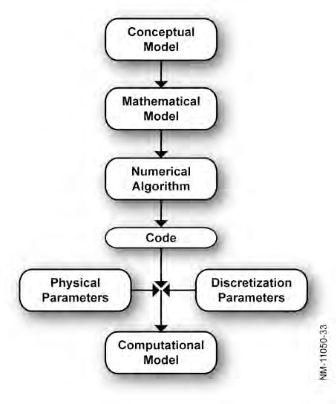
\includegraphics[height=0.6\textheight]{computational-model.png}
    \credit{ASME V\&V 10, \emph{Guide for Verification and Validation in
      Computational Solid Mechanics}.}
  \end{flushleft}
\end{frame}

\begin{frame}{What is an algorithm?}
  \begin{columns}[c]
    \begin{column}{0.62\textwidth}
      ``Informally, an algorithm is any well-defined computational
      \textbf{procedure} that takes some value, or set of values, as
      \textbf{input} and produces some value, or set of values, as
      \textbf{output}.''
      \par\vspace{0.6em}
      \hfill--- Cormen et al.
    \end{column}
    \begin{column}{0.34\textwidth}
      \centering
      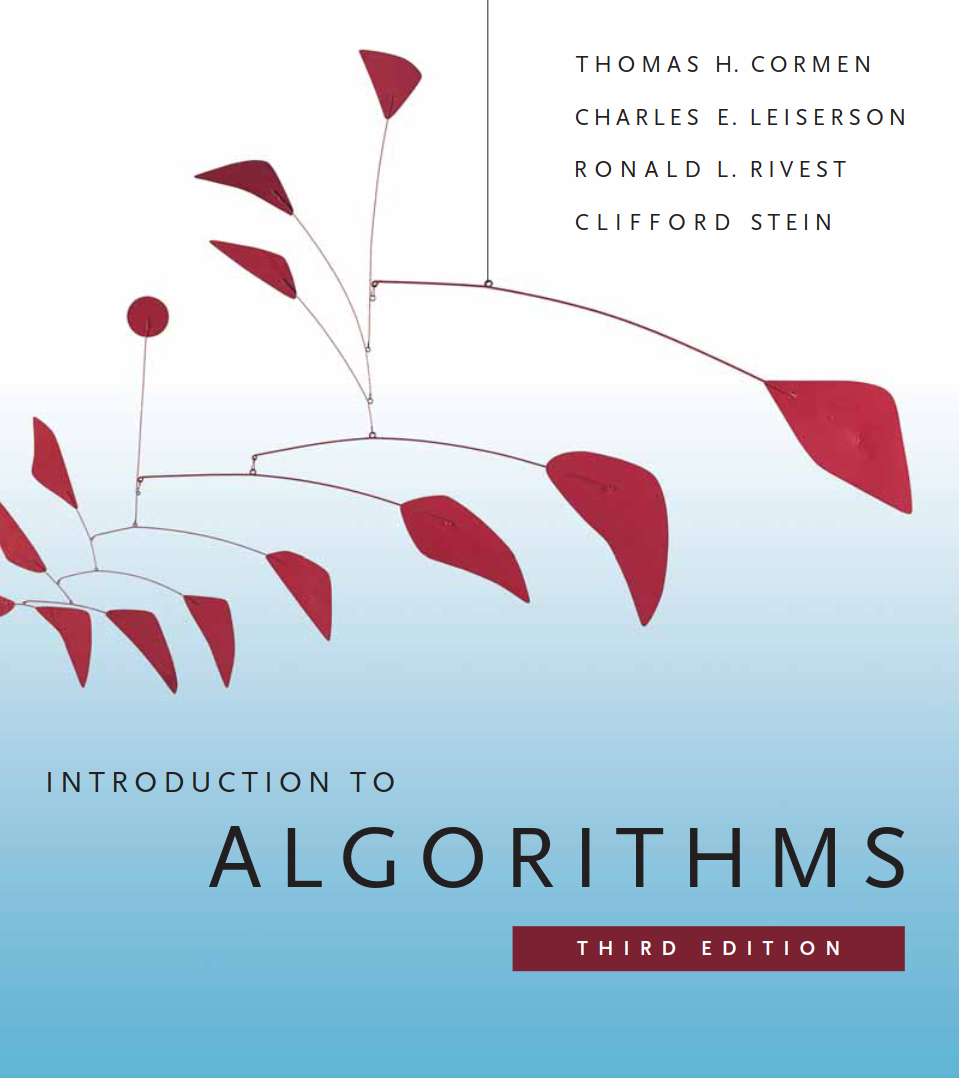
\includegraphics[width=0.8\linewidth]{cormen.png}
      \emph{Introduction to Algorithms}\\
      Cormen, Leiserson,\\ Rivest, and Stein\\[0.8em]
      {\small\href{https://mitpress.mit.edu/9780262046305/}{mitpress.mit.edu}}
    \end{column}
  \end{columns}
\end{frame}

\begin{frame}{Another type of algorithm}
  \begin{center}
    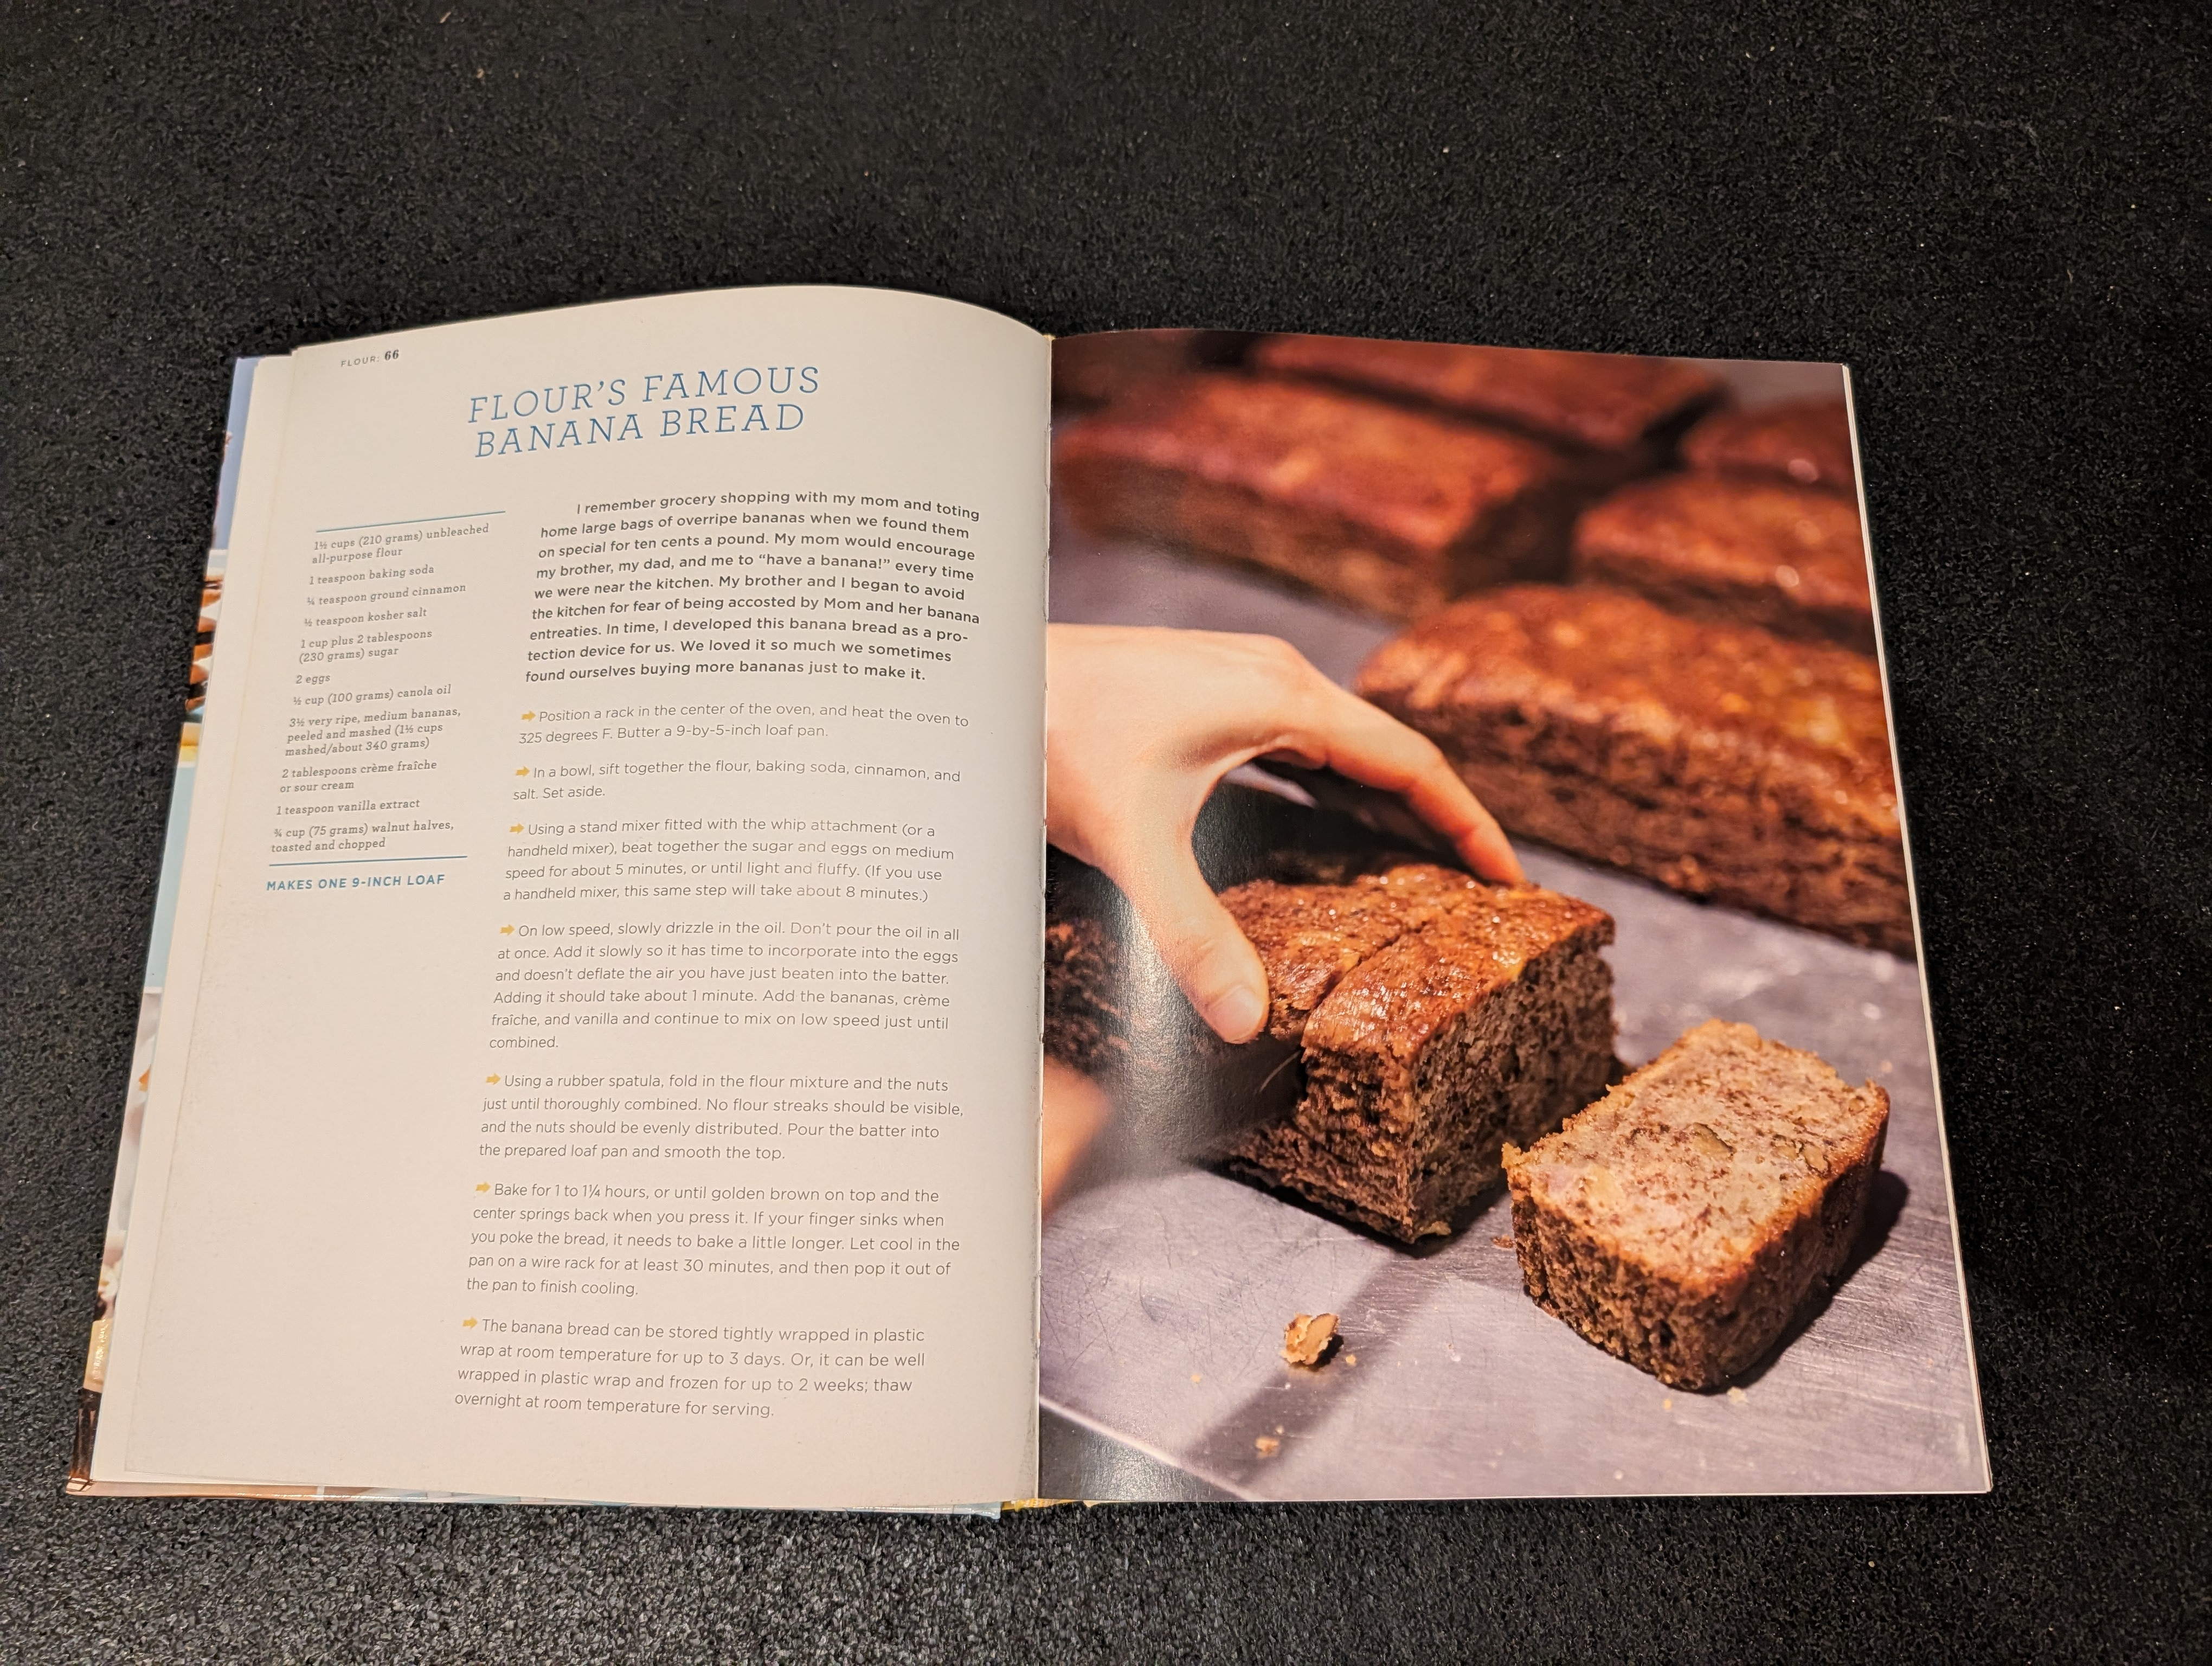
\includegraphics[height=0.85\textheight]{recipe.jpg}
  \end{center}
\end{frame}

\begin{frame}{Why algorithms?}
  \begin{itemize}
    \item Algorithms are mathematical objects. Why are they useful?
        \pause
      \begin{itemize}
        \item We can reason about properties like correctness and resource
          use
          \pause
          \begin{itemize}
            \item[] ``An algorithm is said to be \textbf{correct} if, for
              every input instance, it halts with the correct output.'' --- Cormen et al.
          \end{itemize}
        \pause
        \item We can make precise and rigorous statements without having to
          deal with issues like roundoff error, memory allocation, etc.
      \end{itemize}
  \end{itemize}
\end{frame}

\begin{frame}[fragile]{How do we represent algorithms?}
  \framesubtitle{Matrix-vector multiplication: three ways}
  \begin{columns}[T]
    \begin{column}{0.30\textwidth}
      \centering\textbf{English}\par\vspace{0.5em}
      \raggedright\small
      To get entry $r$ of $\{b\}$, multiply each entry in row $r$ of $[A]$
      by the matching entry of $\{x\}$, and add up the results.
      Do this for every row.
    \end{column}
    \begin{column}{0.32\textwidth}
      \centering\textbf{Code}\par\vspace{0.5em}
\begin{lstlisting}[style=matlab]
b = zeros(n,1);
for r = 1:n
    for c = 1:n
        b(r) = b(r) ...
             + A(r,c)*x(c);
    end
end
\end{lstlisting}
    \end{column}
    \begin{column}{0.34\textwidth}
      \centering\textbf{Pseudocode}\par\vspace{0.5em}
      {\scriptsize% Shared body: \input by matvec-pseudocode.tex (standalone PDF) and by
% algorithms.tex (the slides).  Edit here, both follow.
\begin{algorithm}[H]
  \Input{$n \times n$ matrix $[A]$, vector $\{x\}$}
  \Output{$\{b\} = [A]\{x\}$}
  \BlankLine
  \For{$r \leftarrow 1$ \KwTo $n$}{
    $b[r] \leftarrow 0$\;
    \For{$c \leftarrow 1$ \KwTo $n$}{
      $b[r] \leftarrow b[r] + A[r,c] \cdot x[c]$\;
    }
  }
\end{algorithm}
}
    \end{column}
  \end{columns}
  \vfill
  {\small ``What separates pseudocode from ``real'' code is that in
  pseudocode, we employ whatever expressive method is most clear and concise
  to specify a given algorithm.'' --- Cormen et al.}
\end{frame}

\begin{frame}{Analysis of algorithms}
  \begin{itemize}
    \item \emph{Analyzing} an algorithm means predicting the resources that
      an algorithm requires
      \begin{itemize}
        \item For today, we will count floating point operations
          (``Flops''): multiplication, division, addition, and subtraction
          of floating point numbers
      \end{itemize}
    \item[]
        \pause
    \item \textbf{Discuss with your neighbor:} Consider the equation
      $[A]\{x\} = \{b\}$. As $n$ gets larger, which requires more floating
      point operations? Finding $\{x\}$ given $[A]$ and $\{b\}$, or finding
      $\{b\}$ given $[A]$ and $\{x\}$?
  \end{itemize}
\end{frame}

\begin{frame}{Matrix-vector multiplication}
  \begin{columns}[T]
    \begin{column}{0.52\textwidth}
      {\small% Shared body: \input by matvec-pseudocode.tex (standalone PDF) and by
% algorithms.tex (the slides).  Edit here, both follow.
\begin{algorithm}[H]
  \Input{$n \times n$ matrix $[A]$, vector $\{x\}$}
  \Output{$\{b\} = [A]\{x\}$}
  \BlankLine
  \For{$r \leftarrow 1$ \KwTo $n$}{
    $b[r] \leftarrow 0$\;
    \For{$c \leftarrow 1$ \KwTo $n$}{
      $b[r] \leftarrow b[r] + A[r,c] \cdot x[c]$\;
    }
  }
\end{algorithm}
}
    \end{column}
    \begin{column}{0.44\textwidth}
      % room to write
    \end{column}
  \end{columns}
\end{frame}

\begin{frame}{Gaussian elimination}
  \begin{columns}[T]
    \begin{column}{0.52\textwidth}
      {\scriptsize% Shared body: \input by gauss-pseudocode.tex (standalone PDF) and by
% algorithms.tex (the slides).  Edit here, both follow.
\begin{algorithm}[H]
  \Input{$n \times n$ matrix $[A]$, right-hand side $\{b\}$}
  \Output{solution $\{x\}$ of $[A]\{x\} = \{b\}$}
  \BlankLine
  \tcp{forward elimination}
  \For{$c \leftarrow 1$ \KwTo $n-1$}{
    \For{$r \leftarrow c+1$ \KwTo $n$}{
      $f \leftarrow A[r,c] \,/\, A[c,c]$\;
      \For{$j \leftarrow c$ \KwTo $n$}{
        $A[r,j] \leftarrow A[r,j] - f \cdot A[c,j]$\;
      }
      $b[r] \leftarrow b[r] - f \cdot b[c]$\;
    }
  }
  \BlankLine
  \tcp{back substitution}
  \For{$r \leftarrow n, n-1, \ldots, 1$}{
    $s \leftarrow b[r]$\;
    \For{$j \leftarrow r+1$ \KwTo $n$}{
      $s \leftarrow s - A[r,j] \cdot x[j]$\;
    }
    $x[r] \leftarrow s \,/\, A[r,r]$\;
  }
\end{algorithm}
}
    \end{column}
    \begin{column}{0.44\textwidth}
      % room to write
    \end{column}
  \end{columns}
\end{frame}

\begin{frame}{Asymptotic notation}
  \begin{columns}[T]
    \begin{column}{0.56\textwidth}
      \small
      \begin{itemize}
        \item Asymptotic notation is a tool for keeping track of only the
          terms that are most important as a function approaches an
          asymptote
          \pause
        \item Chapra: $O(m^n)$ means ``terms of order $m^n$ and lower''
      \end{itemize}
      \pause
      \vspace{0.5em}
      \begin{block}{Definition}
        $f(n) = O(g(n))$ as $n \to \infty$ if there exist positive
        constants $c$ and $n_0$ such that
        \vspace{-0.3em}
        \[ 0 \leq f(n) \leq c\,g(n) \quad\text{for all } n \geq n_0 \]
      \end{block}
    \end{column}
    \begin{column}{0.42\textwidth}
      \centering
      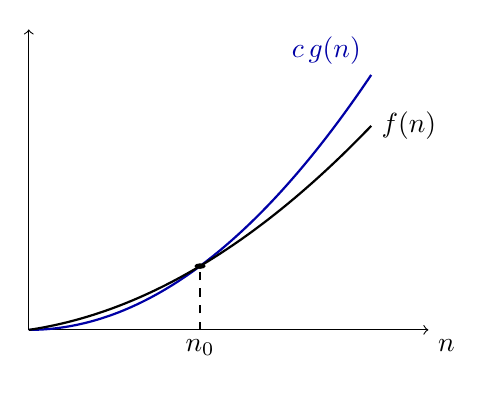
\begin{tikzpicture}[xscale=1.45,yscale=0.72]
        \draw[->] (0,0) -- (3.5,0) node[below right] {$n$};
        \draw[->] (0,0) -- (0,5.3);
        \draw[thick,blue!65!black,domain=0:3,samples=80,smooth]
          plot (\x,{0.5*\x*\x}) node[above left] {$c\,g(n)$};
        \draw[thick,domain=0:3,samples=80,smooth]
          plot (\x,{0.3*\x*\x+0.3*\x}) node[right] {$f(n)$};
        \draw[dashed] (1.5,0) -- (1.5,1.125);
        \fill (1.5,1.125) circle (1.4pt);
        \node[below] at (1.5,0) {$n_0$};
      \end{tikzpicture}
      \par\vspace{0.5em}
      {\small $f(n) \leq c\,g(n)$ for all $n \geq n_0$}
    \end{column}
  \end{columns}
\end{frame}

\begin{frame}{Gaussian elimination}
  \begin{columns}[T]
    \begin{column}{0.52\textwidth}
      {\scriptsize% Shared body: \input by gauss-pseudocode.tex (standalone PDF) and by
% algorithms.tex (the slides).  Edit here, both follow.
\begin{algorithm}[H]
  \Input{$n \times n$ matrix $[A]$, right-hand side $\{b\}$}
  \Output{solution $\{x\}$ of $[A]\{x\} = \{b\}$}
  \BlankLine
  \tcp{forward elimination}
  \For{$c \leftarrow 1$ \KwTo $n-1$}{
    \For{$r \leftarrow c+1$ \KwTo $n$}{
      $f \leftarrow A[r,c] \,/\, A[c,c]$\;
      \For{$j \leftarrow c$ \KwTo $n$}{
        $A[r,j] \leftarrow A[r,j] - f \cdot A[c,j]$\;
      }
      $b[r] \leftarrow b[r] - f \cdot b[c]$\;
    }
  }
  \BlankLine
  \tcp{back substitution}
  \For{$r \leftarrow n, n-1, \ldots, 1$}{
    $s \leftarrow b[r]$\;
    \For{$j \leftarrow r+1$ \KwTo $n$}{
      $s \leftarrow s - A[r,j] \cdot x[j]$\;
    }
    $x[r] \leftarrow s \,/\, A[r,r]$\;
  }
\end{algorithm}
}
    \end{column}
    \begin{column}{0.44\textwidth}
      % room to write
    \end{column}
  \end{columns}
\end{frame}

\end{document}
